\documentclass{../../meta/tudscript}
\begin{document}
\setcounter{section}{9}
\setcounter{subsection}{11}
	\ssect*{Wiederholung Satz: 9.11}
		\begin{enumerate}
		    \item Es existiert ein eindeutig bestimmter ggT$(a,b)$ mit
		        \ilmath{\exists s,t \in \bZ : ggT (a,b)= sa + tb}
		    \item Es existiert ein eindeutig bestimmtes kgV$(a,b)$
		\end{enumerate}

		\sssect{Beweis: 9.11,2 Existenz kgV}
			Ist $a=0$ oder $b=0$, dann ist
			\begin{flalign*}
				kgV (a,b) = 0 \text{ wenn } 0|m \im \exists c \in \bN: m= c \cdot 0 \Rightarrow m = 0
			\end{flalign*}
			Also nehmen wir an, dass $a \neq 0 \land b \neq 0 \im a \cdot b \neq 0$

			\begin{flalign*}
				\text{Sei: } A = \{n \in \bN \{0\} \Big| a|n \land b|n \}
			\end{flalign*}

			Es ist $a \cdot b \in A$, also ist $A$ nicht leer. Nach Satz 9.8 besitzt $A$ ein kleinstes Element, sagen wir $m$.

			Nach Konstruktion ist $a|m \land b|m$.\\

			Sei nun $m' \in \bN \setminus \{0\}$ mit $a|m'$ und $b|m'$.\\
			Nach Lemma 9.9 gibt es $q,r \in \bN$ mit $m' = qm + r$ mit $r < m$.\\

			Mit Proposition 9.2,2 folgt: $a | \underbrace{(m'-qm)}_{r} \land b| \underbrace{(m'-qm)}_{r}$.\\
			Falls $r \neq 0$ dann ist $r \in A$,\\
			da aber $r < m$ ist das ein Widerspruch zur Wahl von M.\\

			Also ist $r = 0$. Dann ist $m|m'$, und $m = kgV (a,b)$\\

			$\hfill\square$

	\ssect{Definition: Teilerfremd}
		Zwei natürliche Zahlen $m,n \in \bN$ heißen \underline{teilerfremd}, wenn $ggT(m,n) = 1$.

	\ssect{Folgerung}
		Seien $m,n,k \in \bN$ wobei $m$ und $n$ teilerfremd sind.

		\begin{flalign*}
			\text{Dann gilt: }m|nk \iff m|k
		\end{flalign*}

		\sssect{Beweis}

			$"\Leftarrow "$
			Übung\textsuperscript{TM} \textit{*Gelächter im ganzen Vorlesungssaal*}

			$"\Rightarrow "$
			Nach Satz 9.11,1 gibt es $s,t \in \bZ$ mit $1=sm+tn$\\
			Da $m|m'$ und $m|m$, folgt nach Proposition 9.2,2:
			\begin{flalign*}
				{m|(ksm +nk) \Rightarrow m|k\underbrace{(sm+tm)}_{1} \implies m|k}
			\end{flalign*}

	\ssect{Bemerkung: Euklidischer Algorithmus}
		Seien $a,b \in \bN$ Berechnung von ggT$(a,b)$ mit Euklidischen Algorithmus:\\

		\textsc{Start}: Setze\\
		$r_0 = a$, $s_0 = 1$, $t_0 = 0$\\
		$r_1 = b$, $s_1 = 0$, $t_1 = 1$\\

		\textsc{Rekursion}: Berechne
		\begin{enumerate}
			\item $q_{n+1}, r_{n+1} \in \bN \text{ mit } r_{n-1} = q_{n+1} \cdot r_n + r_{n+1} \text{ mit } r_{n-1} = r_n$
			\item $s_{n+1} = s_{n-1} - q_{n+1} \cdot s_n$
			\item $t_{n+1} = t_{n-1} - q_{n+1} \cdot t_n$
		\end{enumerate}

		\textsc{Stop}: Falls $r_{n+1} = 0$, mit\\
		$s = s_n, t = t_n, d = r_n$\\

		Man kann nun beweisen, dass ggT$(a,b) = d = sa +tb$

	\ssect{Beispiel: erweiterter Euklidischer Algorithmus}
		$a = 99, b = 78$

		\begin{tabular}{cc|cc}
			q & r  & s & t \\
			\hline
			   & 99 &  1 &  0 \\
			-1 & 78 &  0 &  1 \\
			-3 & 21 &  1 & -1 \\
			-1 & 15 & -3 &  4 \\
			-2 &  6 &  4 & -5 \\
			   &  3 & -11& 14 \\
			\hline
			& 0 & & \\
		\end{tabular}

		Also $ggT (99, 78) = 3 = (-11) \cdot 99 + 14 \cdot 78$

	\ssect{Definition: Verband}
		Anmerkung: Der Satz 9.11 beinhaltet eine wichtige strukturelle Aussage über die geordnete Menge $(\bN, |)$.\\

		Eine geordnete Menge $(M, \leq)$ heißt \underline{Verband}, falls für je zwei Elemente $a,b \in M$ gilt:

		Es gibt in $(M, \leq )$ sowohl Infimum, als auch ein Supremum von $\{a,b\}$

		\sssect{Bemerkung}
			Sei $(M, \leq )$ ein Verband und seien $a,b \in M$. Es bezeichne $a \wedge b$ das
			Infimum von $\{a,b\}$ und $a \vee b$ das Supremum von  $\{a,b\}$

			\begin{enumerate}
				\item Die Abbildungen $\wedge: M \times M \rightarrow M, \vee: M \times M \rightarrow M$ sind assoziativ und kommutativ
				\item Die Strukturen $(M, \wedge)$ und $(M, \vee)$ sind kommutative Halbgruppen.
			\end{enumerate}

			(Wenn M endlich ist, sogar Monoide.)

	\ssect{Folgerung:}

		$(\bN, |)$ ist ein Verband.\\
		Für $a,b \in \bN$ ist ggT (a,b) das Infimum und $\text{kgV}(a,b)$ das Supremum von $\{a,b\}$ in  $(\bN, |)$.

			\sssect{Beweis}
				Das folgt aus Satz 9.11 und Definition von ggT und kgV.\\

				$\hfill\square$

	\ssect{Beispiel}
		$T(50) = \{1, 2, 5, 10, 25, 50\}$\\
		\underline{Teilerdiagramm} von $T(50)$ (Auch Hasse Diagramm genannt)\\

		Vorgehen: Wir zeichnen eine Kante, wenn:
		\begin{enumerate}
			\item $a|b$
			\item es gibt kein $c \in \bN$ mit $a\subset c \subset b$ und $a|c \land c|b$
			\item $a \neq b$
		\end{enumerate}

		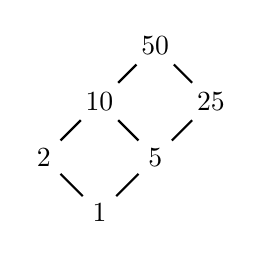
\begin{tikzpicture}
			\node (50) at (0,0) {50};
			\node [below left of=50] (10) {10};
			\node [below right of=50] (25) {25};
			\node [below left of=10] (2) {2};
			\node [below right of=10] (5) {5};
			\node [below left of=5] (1) {1};
			\draw [black,  thick] (50) -- (25);
			\draw [black,  thick] (50) -- (10);
			\draw [black,  thick] (10) -- (2);
			\draw [black,  thick] (10) -- (5);
			\draw [black,  thick] (25) -- (5);
			\draw [black,  thick] (2) -- (1);
			\draw [black,  thick] (5) -- (1);
		\end{tikzpicture}

		Übung: $(T(78),|)$

	\ssect{Definition: Primzahlen}
	Ein natürliche Zahl $n \in \bN \setminus \{0,1\}$ heißt \\

	\underline{prim (Primzahl)} $\iff  T(n) = \{1,n\}$\\
	$\iff \forall a,b \in \bN: n=ab \implies a = 1 \lor b = 1$\\

	Wir bezeichnen die Menge aller Primzahlen mit $\mathbb{P} = \{p \in \bN \setminus \{0,1\} \big| \text{ p prim}\}$.

\end{document}
